\documentclass[a4paper,12pt]{extarticle}
\usepackage[top=3cm]{geometry}

\usepackage{titling}
\setlength{\droptitle}{12em}

\usepackage[scaled]{helvet}
\renewcommand\familydefault{\sfdefault} 
\usepackage[T1]{fontenc}
\usepackage{graphicx}
\usepackage{hyperref}

\usepackage[usenames, dvipsnames]{color}
\definecolor{mygray}{rgb}{0.5, 0.5, 0.5}
\definecolor{mygreen}{rgb}{0,0.6,0}
\definecolor{myblue}{RGB}{57, 135, 189}

\usepackage{listings}
\lstset{ 
    language=java,
    basicstyle=\ttfamily\footnotesize,
    keywordstyle=\color{myblue},
    commentstyle=\color{mygray},
    stringstyle=\color{mygreen},
    frame=single,
    showstringspaces=false,
}

\title{\textbf{Software Engineering\\\vspace{5mm} CPS2002\\\vspace{5mm}  Assignment Report}}

\author{\LARGE Martin Bartolo - 0218300L\vspace{1mm}\\ \LARGE Mikhail Cassar - 0319599M\vspace{3mm}\\ \large BSc (Hons) Computing Science and Mathematics}

\date{Assignment due 27\textsuperscript{th} May 2019}

\setcounter{secnumdepth}{0}

\begin{document}

\setlength{\parindent}{10pt}
\setlength{\footskip}{50pt}
\pagenumbering{arabic}

\maketitle
\thispagestyle{empty}
\newpage

\tableofcontents
\newpage

\section{Diagram Example}
\begin{center}
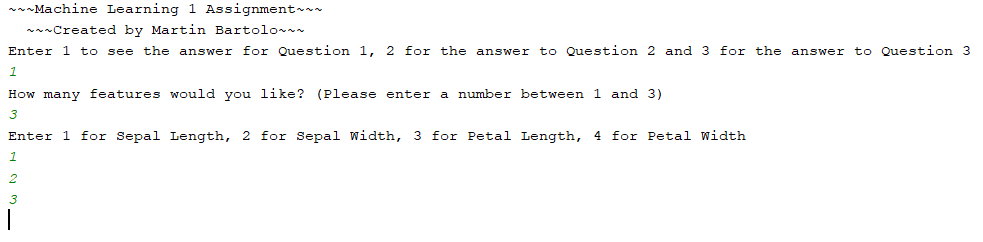
\includegraphics[width=\textwidth]{FigureExample.png}
\end{center}

\section{Code Snippet}
\begin{lstlisting}
public class Main{
  public static void main (String args[]){
    System.out.println("Hello World!");
  }
}
\end{lstlisting}

\section{Introduction}
The aim of this assignment was to collaboratively work on a software project, with the main focus being on rigorous software testing and the use of Git. Our first task was to set up our environments, namely our Git repository on Github and our Jenkins environment on the University Jenkins server. First, we initialised our Git repository and ensured that each team member could commit changes and push and pull them from Github. When this was ensured, we set up our Jenkins environment to work with Maven and scan for changes from Github every few minutes. Whenever changes are found, they are built and run with a detailed code coverage report and test results being displayed using the Emma plug-in. Our progress at this point can be seen by viewing the "Part1" tag on our Github repository. After completing our set-up, we were ready to start working on the two remaining tasks which will be discussed in detail throughout the remainder of this report.
\newpage

<<<<<<< HEAD
\section{Game Design}
The design of the game consists of sectioning the game into the classes, here we will talk about the contents of those classes while also explain how they all work together.
=======
\section{Enhancements}
\subsection{Different Map Types}

The design pattern chosen for this enhancement was the \textbf{factory design pattern}. Since this enhancement was centred around the map's creation then it was clear that a creational design pattern had to be chosen. The main things which needed to be kept in mind were that 2 initial map types had to be implemented while more map types could easily be added to the future. Therefore, the Factory design pattern was the most suitable for the task.\\

The class diagram of the enhancement can be seen below.\\

****Add diagram here****\\
\newpage

\noindent Our implementation is centred around a \textit{Map} interface which contains each method which will be used by the different map types. Each type of map then has a class which implements this main \textit{Map} interface as can be seen in the class diagram above. This design allows for the easy implementation of additional map types in the future.\par

A factory method is present in the \textit{MapCreator} class which is passed the map's type and its size. This class has a creator subclass for every map type, allowing for easy creation of additional map types in the future. An instance of the correct creator subclass will then be made and used to create the map. This can be seen in the code snippet below.

\vspace{-1mm}
\begin{lstlisting}
//Factory Method
Map createMap(String type, int mapSize){

    MapCreator creator;

    if(type.equals("safe")){
        creator = new SafeMapCreator(mapSize);
    }
    else if(type.equals("hazardous")){
        creator = new HazardousMapCreator(mapSize);
    }
    else{
        creator = null;
        System.err.println("Invalid map type");
    }

    if (creator != null) {
        return creator.create();
    }
    else{
        return null;
    }
}
\end{lstlisting}
\vspace{4mm}

\noindent The map is then created in the appropriate creator subclass by setting the map size and calling the generate method in the map type's class (either the \textit{SafeMap} or \textit{HazardousMap} class in our implementation but more can easily be added). A code snippet of this create method for the "safe" map type is shown below

\vspace{-1mm}
\begin{lstlisting}
//Method to create and return a safe map
@Override
public Map create(){
    //getInstance method used here to obtain a 
    //static instance of the hazardous map
    SafeMap map =  SafeMap.getInstance();
    map.setMapSize(mapSize);
    map.generate();
    return map;
}
\end{lstlisting}

\noindent In the generate method for the safe map, the maximum amount of water tiles is set to 10\% and then rounded down to the nearest integer. This code snippet is shown below.

\begin{lstlisting}
//The maximum number of water tiles in a map is set to
//10% of the total tiles
int waterMaxTiles = (int) Math.floor((mapSize*mapSize) * 0.1);
\end{lstlisting}
\vspace{4mm}

\noindent In the generate method for the hazardous map, the maximum amount of water tiles is set to 25\% and then rounded up to the nearest integer. This code snippet is shown below.

\begin{lstlisting}
//The maximum number of water tiles in a map is set to 
//25% of the total tiles
int waterMaxTiles = (int) Math.ceil((mapSize*mapSize) * 0.25);
\end{lstlisting}
\vspace{4mm}

\noindent Apart than these changes, the map is generated as it was in the generate method in the basic version of the program before the enhancements.\\

\noindent When running the program, the user is asked what map type they would like to play with. This can be seen below.

\begin{center}
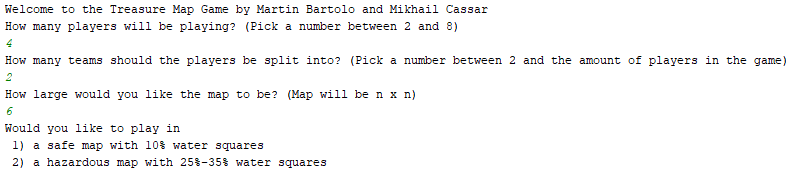
\includegraphics[width=\textwidth]{Figure1.png}
\end{center}

\noindent After the user chooses the map type, the map is created as discussed on the previous page and then the game can be played. On the next page is a comparison between the ending screen of a game played by 4 players in 2 teams on a 6x6 safe map and a game played by the same players on a 6x6 hazardous map. Notice the different amounts of water tiles encountered between the 2 map types.
\newpage

\begin{center}
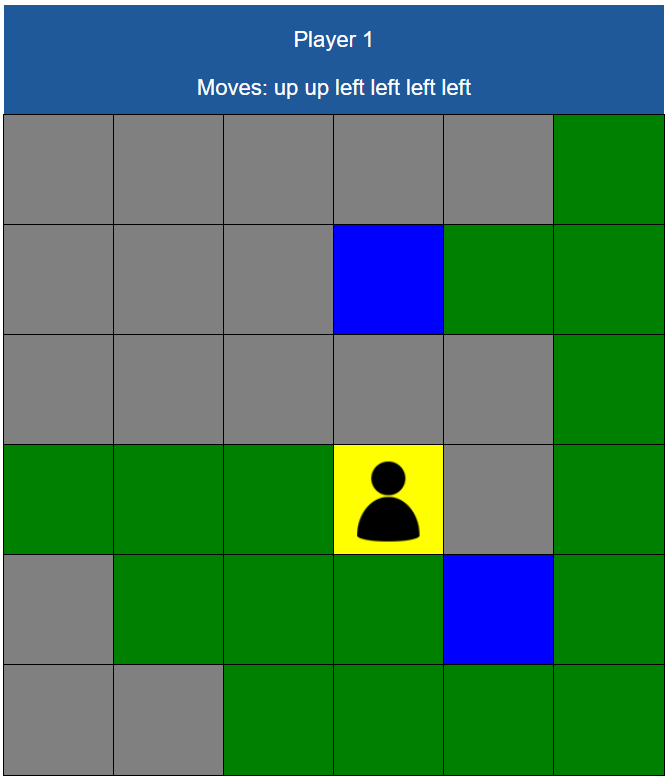
\includegraphics[scale=0.5]{Figure2.png}\\
Ending screen of game using a safe map
\end{center}

\begin{center}
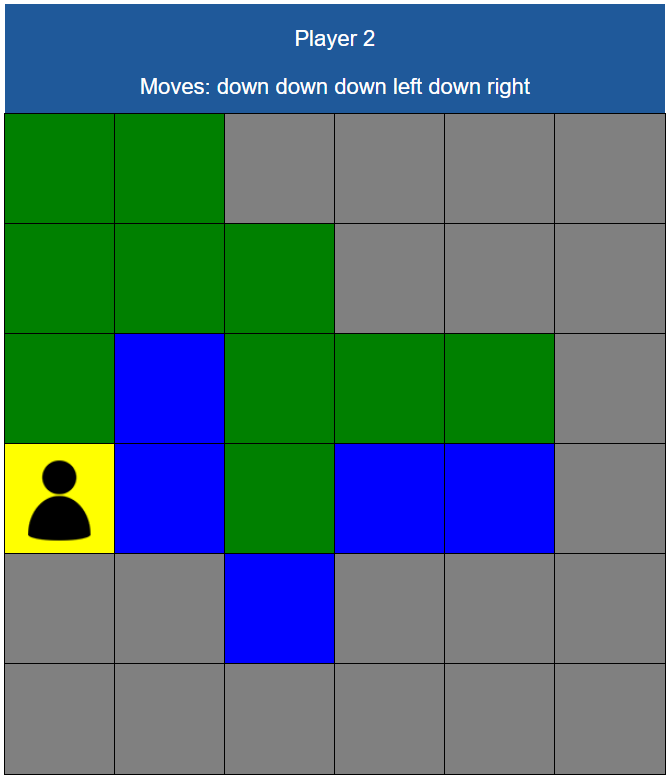
\includegraphics[scale=0.5]{Figure3.png}\\
Ending screen of game using a hazardous map
\end{center}
>>>>>>> 2dc758a53f46e6abe8ec17aa067f8a7bdc40e5f4

The information provided will be regarding the basic version of the game i.e. before any enhancements to the game were made. The basic version of the game can be played by going to the tag "Part2".

\subsection{Class Diagram}
This is the class diagram of the basic version of the game, here one will see how all the classes interact together to provide the user with a functioning game which meets the specified requirements.



\section{Game Enhancements}

\section{Code Coverage Statistics}

\section{Running The Game}


\end{document}
